% Synchronized from AegisKV/design/current_design.md.
% current_design.md is the source of truth; update it before editing this file.
% Source-SHA256: 915886a3fbca8270eb55c1e5867f4c01bff1b0edaa48ab0294972a3392a20682
\section{System Design}
\label{sec:design}

\subsection{Overview}

\system{} has three layers (Figure~\ref{fig:system-overview}).  The application
runtime predicts agent duration and computes Slack.  The serving control plane
contains the Router and Aegis Controller: the Router owns route and output
state, while the Controller incorporates Store Master and owns KV metadata,
protection, recovery order, and protection budgets.  Workers execute inference,
KV movement, and recovery under locally enforced limits.

\begin{figure*}[t]
  \centering
  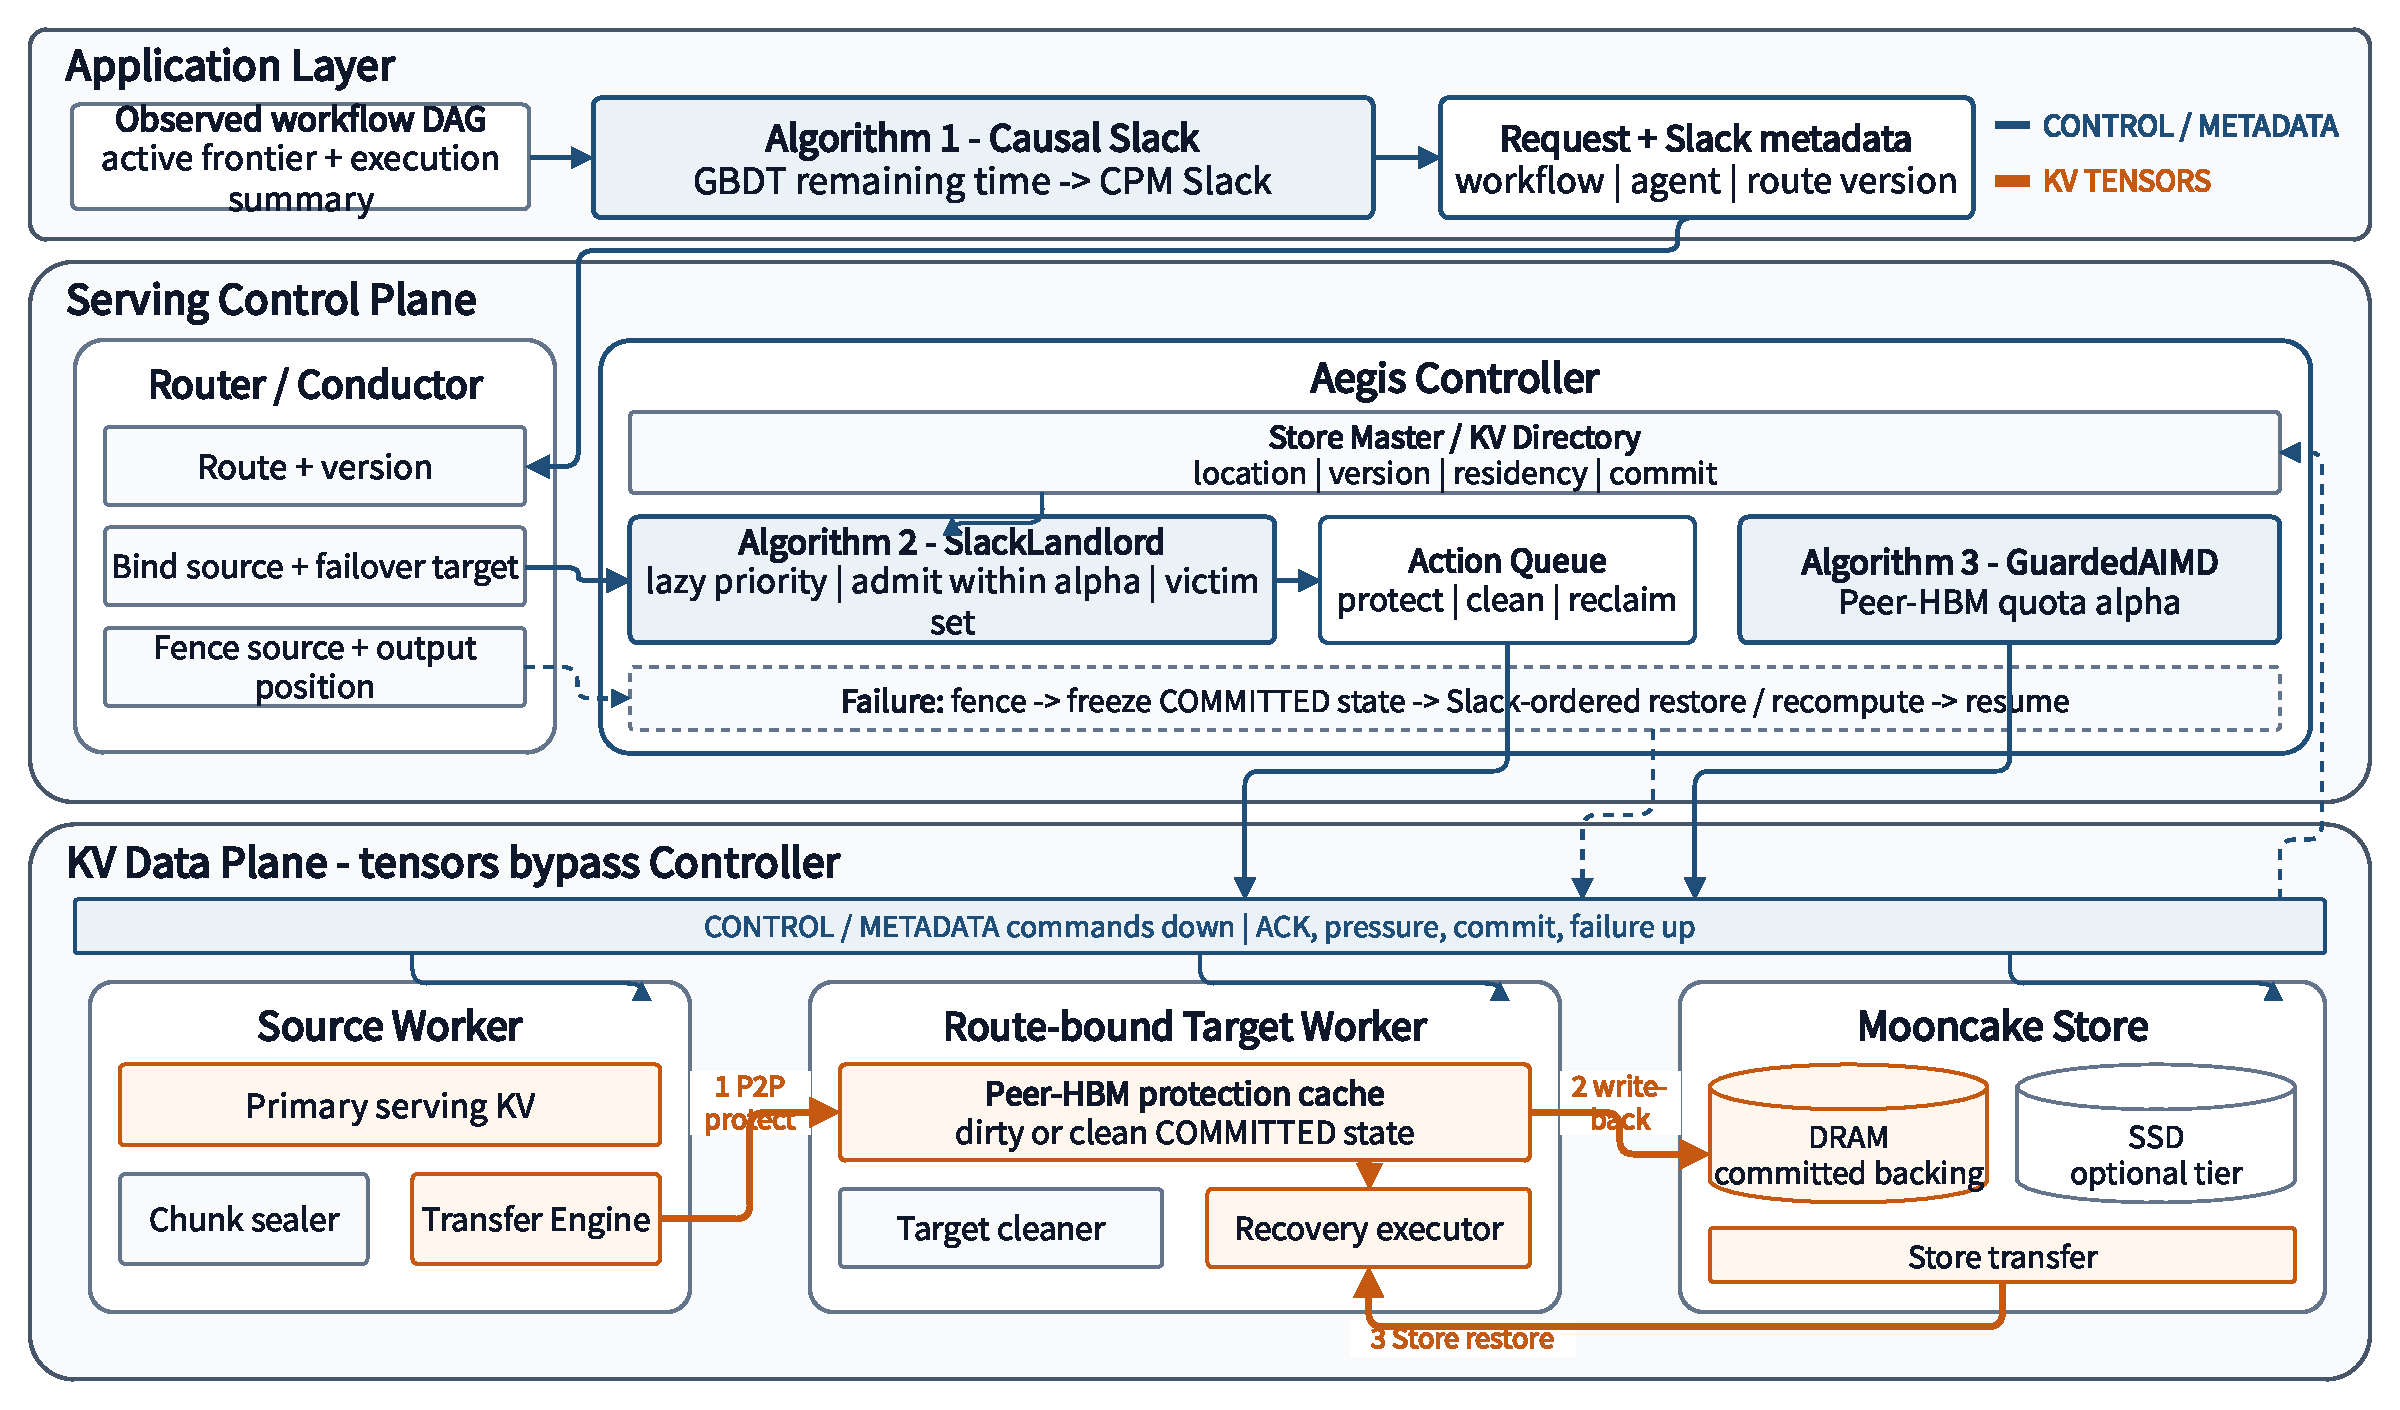
\includegraphics[width=0.89\textwidth]{figures/system-overview.pdf}
  \caption{\system{} overview.  One workflow Slack signal drives normal-period
  protection and failure-time recovery.  Blue arrows carry control and
  metadata; orange arrows carry KV tensors directly among Workers and Store.}
  \Description{A three-layer architecture.  The application layer converts an
  observed workflow DAG into causal Slack metadata.  The serving control plane
  contains the Router, KV Directory, SlackLandlord, action queue, and
  GuardedAIMD.  In the KV data plane, orange paths protect source KV in a
  route-bound target Worker's peer-HBM cache, write committed data back to
  Store DRAM, and restore it to the target after failure; blue paths carry
  commands and acknowledgements.}
  \label{fig:system-overview}
\end{figure*}

Only the application observes agent dependencies, so it computes Slack.  The
Controller has the failure-domain and KV-location view needed by
\textsc{SlackLandlord} and \textsc{GuardedAIMD}; Workers make no global
placement decision.  Persistent \emph{KV Directory} state (chunk locations,
versions, occupancy, and commits) is separated from reconstructible policy
state (pool rent, credit heaps, queues, and control-window counters).

The normal path is short.  A Worker seals a complete KV chunk; the Controller
forms a DRAM candidate or uses the Router-fixed Peer-HBM target; and
\textsc{SlackLandlord} selects bypass or an eviction set from the target's
currently exposed free bytes.  The Controller then evicts that set, allocates
the final space, and records the new chunk as \textsc{Pending}; the action queue
then starts a direct asynchronous copy.  The directory changes it to
\textsc{Committed} only after every shard acknowledges and its version remains
valid.  A failed copy becomes \textsc{Aborted} and releases its space; evicted
replicas are not restored.  On
failure, the Router fences the source and activates a
route-bound target.  The Controller then freezes committed state, chooses
Peer-HBM, DRAM, or recomputation per ready request, and orders recovery with
the same Slack.  KV bytes never pass through the Controller.

\subsection{Application layer: GBDT and CPM}
\label{sec:application-layer}

At each LLM-request or tool-call completion, the workflow runtime uses GBDT to
predict remaining agent durations and runs CPM on the causally revealed
residual DAG from the active frontier to the next join.  If $ES_i$ and $LS_i$
are branch $i$'s earliest and latest starts, the application computes
\begin{equation}
  s_i=[LS_i-ES_i]^+.
  \label{eq:design-slack}
\end{equation}
For one fan-out/join, this reduces to
$[\max_j\widehat T_j-\widehat T_i]^+$.
In Algorithm~\ref{alg:slack-update}, $\mathcal N_t$ is the set of visible
agent nodes, $\mathcal A_t$ is the active frontier, and
$\mathcal V_t^{\mathrm{start}}$ and $\mathcal V_t^{\mathrm{end}}$ are the
start and end nodes.  An active node uses predicted remaining duration, a visible
not-yet-started node uses predicted full duration, and a structural node has
zero weight.
It attaches $s_i$ to the next request as ordinary metadata.  The Controller
decreases it by elapsed request time, and the next application update replaces
the old value.  Missing Slack, an incomplete residual sub-DAG, or a missing
node prediction yields zero Slack.  Prediction error changes priority but
cannot violate resource or recovery safety.

Algorithm~\ref{alg:slack-update} shows the complete online path.  On each
request or tool return, \textsc{UpdateSlack} records the event (line 1), orders
the residual DAG and identifies its start and end nodes (line 2), then predicts
visible node weights in an explicit loop (lines 3--5).  The forward loop
computes earliest starts in topological order (lines 6--8).  The end-node
completion span initializes the backward loops, which compute latest starts in
reverse topological order (lines 9--14).  A final loop computes, validates,
stores, and attaches active-branch Slack (lines 15--17).  Repeated returns
therefore revise Slack causally; the algorithm never reads a future output
length, completion time, or failure location.

For fixed $G_t$ and nonnegative predicted weights, the two passes compute exact
CPM total float on that residual DAG.  This is not a guarantee of true future
Slack; incomplete inputs fail closed to zero and later returns revise the estimate.

For $N$ visible agent nodes, $F$ features, $M$ depth-$d$ trees, and residual
DAG $G_t=(V_t,E_t)$, one update costs
$O(N(F+Md)+|V_t|+|E_t|)$ time and $O(|V_t|+|E_t|)$ state excluding the fixed
model.  With a fixed feature schema and model, time is
$O(|V_t|+|E_t|)$ and is paid only on a request or tool return, not per token.

% Compiled by sections/03-system-design-v2.tex.
% Design-SHA256: 915886a3fbca8270eb55c1e5867f4c01bff1b0edaa48ab0294972a3392a20682
\begin{algorithm}[t]
\caption{Online GBDT--CPM Slack update}
\label{alg:slack-update}
\begin{tabular}{@{}r@{\hspace{0.5em}}>{\raggedright\arraybackslash}p{\dimexpr\columnwidth-2.5em\relax}@{}}
\multicolumn{2}{@{}>{\raggedright\arraybackslash}p{\columnwidth}@{}}{\textbf{UpdateSlack}$(e,t)$}\\
\multicolumn{2}{@{}>{\raggedright\arraybackslash}p{\columnwidth}@{}}{\textit{Symbols.} $G_t=(V_t,E_t)$: residual DAG; $H_t$: execution summary; $\mathcal N_t/\mathcal A_t$: agent nodes/active frontier; $\mathcal V_t^{\mathrm{start}}/\mathcal V_t^{\mathrm{end}}$: start/end-node sets.}\\
\multicolumn{2}{@{}>{\raggedright\arraybackslash}p{\columnwidth}@{}}{$f_\theta/\phi_v$: GBDT/features; $\hat w_v$: predicted time; $ES_v/LS_v$: earliest/latest start; $\sigma_i=(s_i,t)$; $\operatorname{Valid}_i$: complete causal input.}\\
1 & $(G_t=(V_t,E_t),H_t,\mathcal N_t,\mathcal A_t)\gets\operatorname{Observe}(G_{t^-},H_{t^-},e)$.\\
2 & $\pi\gets\operatorname{Topo}(G_t)$; $\mathcal V_t^{\mathrm{start}}\gets\{v:\operatorname{pred}(v)=\varnothing\}$; $\mathcal V_t^{\mathrm{end}}\gets\{v:\operatorname{succ}(v)=\varnothing\}$.\\
3 & \textbf{for} $v\in V_t$ \textbf{do}\\
4 & $\quad\hat w_v\gets0$; \textbf{if} $v\in\mathcal N_t$ \textbf{then} $\hat w_v\gets f_\theta(\phi_v(G_t,H_t))$.\\
5 & \textbf{end for}\\
6 & \textbf{for} $v\in\pi$ \textbf{do}\\
7 & $\quad$\textbf{if} $v\in\mathcal V_t^{\mathrm{start}}$ \textbf{then} $ES_v\gets0$; \textbf{else} $ES_v\gets\max_{u\in\operatorname{pred}(v)}(ES_u+\hat w_u)$.\\
8 & \textbf{end for}\\
9 & $C_t\gets\max_{v\in\mathcal V_t^{\mathrm{end}}}(ES_v+\hat w_v)$.\\
10 & \textbf{for} $v\in\mathcal V_t^{\mathrm{end}}$ \textbf{do} $LS_v\gets C_t-\hat w_v$.\\
11 & \textbf{end for}\\
12 & \textbf{for} $v\in\operatorname{rev}(\pi)\setminus\mathcal V_t^{\mathrm{end}}$ \textbf{do}\\
13 & $\quad LS_v\gets\min_{u\in\operatorname{succ}(v)}LS_u-\hat w_v$.\\
14 & \textbf{end for}\\
15 & \textbf{for} $i\in\mathcal A_t$ \textbf{do}\\
16 & $\quad s_i\gets[LS_i-ES_i]^+$; $\neg\operatorname{Valid}_i\Rightarrow s_i\gets0$; $\sigma_i\gets(s_i,t)$; $\operatorname{meta}(\operatorname{next}(i))[s]\gets s_i$.\\
17 & \textbf{end for}\\
\end{tabular}
\end{algorithm}


\subsection{Serving control plane}
\label{sec:control-plane}

\subsubsection{Router and Conductor}

The Router tracks request-to-Worker mappings, Worker health, route versions,
and committed output positions.  Each route version binds a model, KV ABI,
parallel layout, and compatible failover target.  Peer-HBM protection is
created only on that target.  On failure, the Router fences the source, freezes
output, and activates the target.  A later target may use failure-domain-safe
DRAM, but cannot use Peer HBM belonging to the failed route.

\subsubsection{Aegis Controller}

The Controller incorporates Store Master.  Its KV Directory tracks each
chunk's source domain, route version, completeness, location, and bytes.
Store Master checks the model, KV ABI, parallel layout, and failure domain and
maps a chunk to logical DRAM.  The Router already fixes each request's
Peer-HBM target.  Algorithm 2 therefore receives an already-targeted placement
instead of enumerating pools.  Each target Worker keeps independent HBM
capacity, rent, and heap state.

\paragraph{SlackLandlord.}
Classic Landlord assigns object credit and evicts the object whose normalized
credit is exhausted first~\cite{young2002online}.  \textsc{SlackLandlord} keeps
this credit/rent mechanism but applies it to variable-size KV chunks in DRAM
and Peer HBM.

\textbf{KV chunks.}
Request KV is divided in token order.  The default prefix chunk is 4096 tokens
and the default decode chunk is 256 tokens:
\begin{equation}
 q_{P}=4096,\qquad q_{D}=256.
 \label{eq:chunk-granularity}
\end{equation}
These are configurable implementation parameters; every capacity check uses
the actual bytes $b_c$, which depend on the realized token count, model, KV
type, and parallel layout.  A sealed chunk contains all TP/PP shards for its
token interval.  An open decode tail is not protected until it reaches its
boundary.  Request $i$ maintains DRAM and Peer-HBM frontiers $f_i^D$ and
$f_i^H$.  Admission advances one frontier; eviction removes its suffix tail.
Peer HBM requires the same chunk in DRAM, and deleting a DRAM tail also deletes
its HBM overlay.  Hence both tiers always hold complete continuous prefixes.

\textbf{Recovery harm and credit.}
For committed state $S_i$, a constant-time estimator compares full
recomputation, DRAM, and Peer-HBM recovery, including the slowest shard,
unprotected suffix, and silent replay.  Its Slack-visible harm is
\begin{equation}
 J_i(S_i,t)=[T_i(S_i)-s_i(t)]^+.
 \label{eq:recovery-harm}
\end{equation}
Candidate $x=(c,r)$ targets either DRAM or the Router-fixed Peer-HBM Worker and
receives admission credit
\begin{equation}
 A_x=[J_i(S_i,t)-J_i(S_i\oplus x,t)]^+.
 \label{eq:chunk-credit}
\end{equation}
\textsc{Gain}$(x,t)$ returns this value.  For a tentative eviction set $Y$,
\textsc{Loss}$(Y,t)$ directly compares the affected requests before and after
legal suffix removal and returns joint loss $D_Y$.  Removing a DRAM chunk also
removes its HBM overlay.  No separate per-chunk conditional-loss symbol is
needed.

\textbf{Credit and rent.}
Each pool $r$ has cumulative rent $L_r$ and one min-heap $Q_r$.  Every resident
chunk retains its key, while $Q_r$ exposes at most one currently evictable
suffix tail per request.  Candidate $c$ committed at rent $L_r'$ receives
\begin{equation}
 H_c=L_r'+A_x/b_c,
 \qquad \Theta_x=L_r+A_x/b_c,
 \label{eq:landlord-credit}
\end{equation}
where $b_y[H_y-L_r]^+$ is resident $y$'s remaining credit and $\Theta_x$ is
candidate $x$'s threshold.  A hidden chunk keeps its key instead of receiving
fresh credit when it becomes a tail again.  A Slack update changes only that
request's indexed tail entry; a hidden key is refreshed when exposed:
$H_y\leftarrow\max\{L_r,H_y+(D^{new}-D^{old})/b_y\}$.

The algorithm reads the target's currently exposed free bytes
$f=\operatorname{Free}(r)$.  While $f<b_c$, it tentatively removes minimum-key
tails from other requests and adds their bytes to $f$.  Excluding the
candidate's request preserves its prefix prerequisites.  Every selected key must remain below
$\Theta_x$, and admission credit must exceed the joint loss $D_Y$.  The Controller then immediately
evicts $Y$, advances rent to $\max_{y\in Y}H_y$, allocates the final space, and
marks the candidate \textsc{Pending}.  The copy then proceeds asynchronously;
failure frees its space but does not restore $Y$.
Thus a 4096-token prefix chunk may replace up to roughly sixteen 256-token
decode chunks instead of relying on an invalid one-object exchange.

% Compiled by sections/03-system-design-v2.tex.
% Design-SHA256: 915886a3fbca8270eb55c1e5867f4c01bff1b0edaa48ab0294972a3392a20682
\begin{algorithm}[t]
\caption{\textsc{SlackLandlord}}
\label{alg:slack-landlord}
\begin{tabular}{@{}r@{\hspace{0.5em}}>{\raggedright\arraybackslash}p{\dimexpr\columnwidth-2.5em\relax}@{}}
\multicolumn{2}{@{}>{\raggedright\arraybackslash}p{\columnwidth}@{}}{\textit{Symbols.} $x=(c,r)$: candidate chunk $c$ ($b_c$ bytes) and target $r$; $i=\operatorname{req}(c)$.}\\
\multicolumn{2}{@{}>{\raggedright\arraybackslash}p{\columnwidth}@{}}{$L_r$: rent; $Q_r$: tail min-heap keyed by $H_y$; $Y$: tentative evictions; $Q$: temporary view of $Q_r$.}\\
\multicolumn{2}{@{}>{\raggedright\arraybackslash}p{\columnwidth}@{}}{$f$: free bytes exposed by target $r$; $\bot$: none.}\\
\multicolumn{2}{@{}>{\raggedright\arraybackslash}p{\columnwidth}@{}}{\textbf{SlackLandlord}$(x=(c,r),t)$}\\
1 & $A\gets\operatorname{Gain}(x,t)$; $\Theta\gets L_r+A/b_c$; $Y\gets\varnothing$; $Q\gets\operatorname{View}(Q_r)$.\\
2 & $f\gets\operatorname{Free}(r)$.\\
3 & \textbf{while} $f<b_c$ \textbf{do}\\
4 & $\quad(y,H_y)\gets\operatorname{MinTail}(Q,Y,i,t)$.\\
5 & $\quad$\textbf{if} $(y=\bot)\lor(H_y\ge\Theta)$ \textbf{then} \textbf{return} \textsc{Bypass}.\\
6 & $\quad Y\gets Y\cup\{y\}$; $f\gets f+b_y$.\\
7 & $\quad z\gets\operatorname{PrevTail}(y,Y)$; $z\ne\bot\Rightarrow Q.\operatorname{insert}(z,\operatorname{RefreshKey}(z,Y,t))$.\\
8 & \textbf{end while}\\
9 & $D\gets\operatorname{Loss}(Y,t)$; $A\le D\Rightarrow\operatorname{return}\ \textsc{Bypass}$.\\
10 & $\operatorname{Evict}(Y)$; $Y\ne\varnothing\Rightarrow L_r\gets\max\{L_r,\max_{y\in Y}H_y\}$.\\
11 & $\operatorname{Allocate}(c,r,b_c)$; $\operatorname{state}(c)\gets\textsc{Pending}$.\\
12 & $\operatorname{Transfer.Enqueue}(x)$; $\operatorname{return}\ \textsc{Pending}$.\\
\multicolumn{2}{@{}>{\raggedright\arraybackslash}p{\columnwidth}@{}}{\textbf{MinTail}$(Q,Y,i,t)$}\\
13 & \textbf{while} $Q\ne\varnothing$ \textbf{do}\\
14 & $\quad(y,H_y)\gets Q.\operatorname{min}()$.\\
15 & $\quad$\textbf{if} $\operatorname{Stale}(y,Y,t)$ \textbf{then} $Q.\operatorname{update}(y,\operatorname{RefreshKey}(y,Y,t))$; \textbf{continue}.\\
16 & $\quad Q.\operatorname{pop}()$; $\operatorname{req}(y)\ne i\Rightarrow\operatorname{return}\ (y,H_y)$.\\
17 & \textbf{end while}; $\operatorname{return}\ (\bot,\infty)$.\\
\multicolumn{2}{@{}>{\raggedright\arraybackslash}p{\columnwidth}@{}}{\textbf{OnCopyDone}$(x=(c,r),t')$}\\
18 & \textbf{if} $\operatorname{AllAck}(c)\land\operatorname{Valid}(c)$ \textbf{then}\\
19 & $\quad H_c\gets L_r+\operatorname{Gain}(x,t')/b_c$; $\operatorname{state}(c)\gets\textsc{Committed}$; $Q_r.\operatorname{insert}(c,H_c)$; \textbf{return}.\\
20 & $\operatorname{state}(c)\gets\textsc{Aborted}$; $\operatorname{Free}(c)$.\\
\end{tabular}
\end{algorithm}


Algorithm~\ref{alg:slack-landlord} combines selection and installation in one
normal-period procedure for one already-targeted candidate.  Line 1 computes
its Slack-aware gain and Landlord threshold and creates a temporary view of
$Q_r$.  Line 2 reads the target's current free-space snapshot.  Lines 3--8
gather enough bytes: after
selecting tail $y$, line 7 inserts the same request's newly exposed predecessor.
\textsc{MinTail} (lines 13--17)
repeatedly refreshes a stale heap top, then returns the stable minimum while
skipping the candidate's own request.  Because $Q_r$ contains only the current
safe suffix tail of each request, no pool-wide scan is needed.  Line 9 requires
the admission gain to exceed $Y$'s joint loss.  Lines 10--11 immediately evict
$Y$, advance rent, allocate the candidate's final space, and mark it
\textsc{Pending}; line 12 starts the direct
copy through the Transfer Engine and returns.  The completion callback
(lines 18--20) commits only a complete, version-valid chunk, or aborts it and
frees its space.  Transfer queueing and token accounting remain inside the
existing Transfer Engine.  The Store Master orders
these short metadata updates per pool, but does not stage $Y$, wait under a
pool lock, roll back an eviction, or run an old/new replacement transaction.
Calls and capacity updates for one pool are serialized through its metadata
queue, so one call uses the free-space snapshot read by line 2 and
concurrent requests cannot consume the same free-space or heap snapshot; different pools
and all KV transfers remain parallel.
Failure-time recovery is deliberately outside Algorithm 2.

For $R$ active requests, $k=|Y|$ selected chunks, $u$ stale-key refreshes, and
$m$ shards, heap pops, updates, and predecessor insertions each cost
$O(\log(R+1))$.  \textsc{Loss} costs $O(k)$ with the frontier estimator, while
install and completion touch at most $m$ shard records.  Algorithm 2 therefore
costs
\begin{equation}
 O\bigl((k+u+1)\log(R+1)+k+m\bigr)
 \label{eq:slack-landlord-cost}
\end{equation}
of Controller time.  A key is refreshed at most once per Slack/frontier epoch,
giving the conservative per-call bound $u=O(R+k)$.  Under the default 4096/256
sizes and a fixed model/layout, a full prefix needs at most sixteen full decode
chunks.  The persistent heap uses $O(R)$ state, a copy-on-write temporary view
records $O(k+u)$ changes, and saved keys and versions use $O(C)$ chunk metadata.
Copying remains asynchronous and is outside this bound.  Only complete,
version-valid chunks become
\textsc{Committed}, and a \textsc{Pending} chunk is never used for recovery.
The algorithm deliberately permits a protection gap between evicting $Y$ and
committing the new chunk; a failure in this interval falls back to another
committed tier or recomputation.  It does not claim the global optimum or a new
competitive ratio.

In a Mooncake-style implementation, \textsc{SlackLandlord} is a policy module inside
the existing Store Master.  Segment allocation, batch-put completion, and
eviction hooks are sufficient; Peer-HBM mappings remain in the serving
framework and Transfer Engine.

\paragraph{Alpha control}
Algorithm~\ref{alg:guarded-aimd} updates only the shadow-HBM fraction $\alpha_p$ for each
Router-fixed Peer-HBM target $p$.  It neither selects chunks nor controls paths.
For target capacity $M_p$, the published shadow-KV quota is $\alpha_pM_p$.
HBM pressure $q_p=1$ reports insufficient primary headroom or an
allocation/reclaim stall.  With stable-window counter $z_p$, decrease factor
$0<\gamma<1$, additive step $\delta>0$, and stable threshold $K$, the update is
\begin{equation}
 (\alpha_p',z_p')=
 \begin{cases}
 (\max\{\alpha_p^{min},\gamma\alpha_p\},0),&q_p=1,\\
 (\min\{\alpha_p^{max},\alpha_p+\delta\},0),&q_p=0\land z_p+1\ge K,\\
 (\alpha_p,z_p+1),&\text{otherwise}.
 \end{cases}
 \label{eq:guarded-aimd}
\end{equation}

% Compiled by sections/03-system-design-v2.tex.
% Design-SHA256: 915886a3fbca8270eb55c1e5867f4c01bff1b0edaa48ab0294972a3392a20682
\begin{algorithm}[b]
\caption{\textsc{GuardedAIMD}: Peer-HBM share}
\label{alg:guarded-aimd}
\begin{tabular}{@{}r@{\hspace{0.5em}}>{\raggedright\arraybackslash}p{\dimexpr\columnwidth-2.5em\relax}@{}}
\multicolumn{2}{@{}>{\raggedright\arraybackslash}p{\columnwidth}@{}}{\textit{Symbols.} $p$: Peer-HBM target; $\alpha_p$: shadow-HBM fraction; $q_p\in\{0,1\}$: HBM pressure; $z_p$: stable windows.}\\
\multicolumn{2}{@{}>{\raggedright\arraybackslash}p{\columnwidth}@{}}{$0<\gamma<1$: decrease factor; $\delta>0$: increase step; $K$: stable-window threshold; $[\alpha_p^{min},\alpha_p^{max}]$: bounds.}\\
\multicolumn{2}{@{}>{\raggedright\arraybackslash}p{\columnwidth}@{}}{\textbf{ControlWindow}$(t)$}\\
1 & \textbf{for} $p\in\mathcal P$ \textbf{do}\\
2 & $\quad$\textbf{if} $q_p=1$ \textbf{then}\\
3 & $\qquad\alpha_p\gets\max\{\alpha_p^{min},\gamma\alpha_p\}$; $z_p\gets0$.\\
4 & $\quad$\textbf{else} $z_p\gets z_p+1$.\\
5 & $\qquad z_p\ge K\Rightarrow(\alpha_p,z_p)\gets(\min\{\alpha_p^{max},\alpha_p+\delta\},0)$.\\
6 & $\quad$\textbf{end if}; $\operatorname{Publish}(p,\alpha_p,t)$.\\
7 & \textbf{end for}\\
\end{tabular}
\end{algorithm}


Lines 1--7 iterate over targets, update only $\alpha_p$, and publish the next
window's value.  If a new $\alpha_pM_p$ is below current shadow use, the Worker
blocks new Peer-HBM admission and emits a capacity-change event; Store Master
reclaims suffix tails in SlackLandlord key order.  This is enforcement of the
published quota, not a second decision inside Algorithm 3.  Transfer queueing,
rate control, and token release remain in the Transfer Engine.  For $P$ peer
targets, one control window costs $O(P)$ time and $O(P)$ state and does not
enter chunk admission or per-token decode.

\subsection{Worker layer}
\label{sec:worker-layer}

Each Worker contains a KV Manager, Transfer Engine, local resource enforcer,
and Recovery Executor.  The KV Manager uses 4096-token prefix chunks and
256-token decode chunks by default; an open decode tail is recomputed.  The
Transfer Engine copies KV to peer HBM, writes or loads Store KV, and owns copy
queueing, rate control, and tokens without sending bytes through the Controller.
The local resource enforcer applies the $\alpha_pM_p$ quota; the existing
allocator independently protects primary allocations and serving reserve.  Peer shadows are
private before failure and cannot become normal prefix-cache hits.  Recovery
adopts only complete, version-compatible chunks.

Before sending output, the Router records the accepted output position.
Recovery silently replays the gap between the last complete KV boundary and
that position.  All ranks finish before the Router restores route and output
authority, preventing partial adoption and duplicate output.

\subsection{End-to-end scope}
\label{sec:end-to-end}

The first implementation handles one fail-stop GPU process, GPU, or host at a
time and assumes the application, Router, persistent KV Directory, network,
and a compatible Worker survive.  It first supports a DP replica with the same
model revision, KV ABI, and parallel layout.  PP requires every stage and TP
every rank; unsupported layouts fail closed and restart.

GBDT, CPM, Landlord, and AIMD are building blocks.  The contribution is the
cross-layer mechanism that applies one request-level Slack and one fail-now
recovery model twice: \textsc{SlackLandlord} turns them into normal-period KV
chunk admission and eviction credits, while failure recovery turns them into due times.
\textsc{GuardedAIMD} adjusts only the slow-timescale Peer-HBM alpha envelope;
the Worker enforces its local cap without placing foreground inference safety
in the Controller's critical path.
